\documentclass[aspectratio=169]{beamer}

\usetheme{Madrid}
\usecolortheme{default}

\usefonttheme{professionalfonts}
\usepackage[T1]{fontenc}
\usepackage[type1]{ebgaramond}
\usepackage[scale=0.95,semibold]{montserrat}
\renewcommand{\familydefault}{\sfdefault}
\newcommand{\oliveDisplayFont}{\ebgaramond\mdseries\upshape}
\newcommand{\oliveTitleFont}{\oliveDisplayFont\scshape}
\setbeamerfont{title}{size={\fontsize{21}{23}},series=\mdseries,family=\oliveDisplayFont}
\setbeamerfont{frametitle}{size=\large,series=\mdseries,family=\oliveTitleFont}
\setbeamerfont{subtitle}{size=\large,series=\mdseries,family=\oliveDisplayFont}
\setbeamerfont{author}{size=\Large,series=\mdseries,family=\oliveDisplayFont}
\setbeamerfont{institute}{size=\small,series=\mdseries,family=\oliveDisplayFont}
\setbeamerfont{date}{size=\scriptsize,series=\mdseries,family=\oliveDisplayFont}

\definecolor{oliveGreen}{HTML}{5A7411}
\definecolor{oliveDark}{HTML}{3C4D0B}
\definecolor{oliveCream}{HTML}{F0EEDC}
\definecolor{olivePale}{HTML}{DDE3C2}
\definecolor{oliveRust}{HTML}{C1502E}
\definecolor{oliveRustBg}{HTML}{F8ECE4}
\definecolor{oliveTeal}{HTML}{2F6F73}
\definecolor{oliveTealBg}{HTML}{E7F0F0}
\definecolor{oliveInk}{HTML}{1A1A1A}
\definecolor{olivePaper}{HTML}{F8F6F2}
\definecolor{oliveBoxHeading}{HTML}{E4E9D8}
\definecolor{oliveBoxBody}{HTML}{F1F3EB}
\setbeamercolor{normal text}{fg=oliveInk,bg=olivePaper}
\setbeamercolor{structure}{fg=oliveGreen}
\setbeamercolor{palette primary}{fg=oliveCream,bg=oliveGreen}
\setbeamercolor{palette secondary}{fg=oliveCream,bg=oliveDark}
\setbeamercolor{palette tertiary}{fg=oliveCream,bg=oliveGreen}
\setbeamercolor{palette quaternary}{fg=oliveCream,bg=oliveDark}
\setbeamercolor{title}{fg=oliveCream,bg=oliveGreen}
\setbeamercolor{subtitle}{fg=olivePale}
\setbeamercolor{frametitle}{fg=oliveCream,bg=oliveGreen}
\setbeamercolor{framesubtitle}{fg=olivePale}
\setbeamertemplate{blocks}[rounded][shadow=false]
\setbeamercolor{block title}{fg=oliveDark,bg=oliveBoxHeading}
\setbeamercolor{block body}{fg=oliveInk,bg=oliveBoxBody}
\setbeamercolor{block title alerted}{fg=oliveRust!75!oliveInk,bg=oliveRust!12!olivePaper}
\setbeamercolor{block body alerted}{fg=oliveInk,bg=oliveRust!4!olivePaper}
\setbeamercolor{block title example}{fg=oliveTeal!75!oliveInk,bg=oliveTeal!12!olivePaper}
\setbeamercolor{block body example}{fg=oliveInk,bg=oliveTeal!4!olivePaper}
\setbeamercolor{alerted text}{fg=oliveRust}
\setbeamercolor{example text}{fg=oliveTeal}
\hypersetup{urlcolor=oliveGreen,linkcolor=oliveGreen,citecolor=oliveGreen}
\usepackage{amsmath}
\usepackage{algorithm}
\usepackage{algpseudocode}
\usepackage{booktabs}
\usepackage{graphicx}
\usepackage{tikz}
\usetikzlibrary{shapes.geometric, arrows.meta, positioning, fit}

\setbeamertemplate{background}{%
  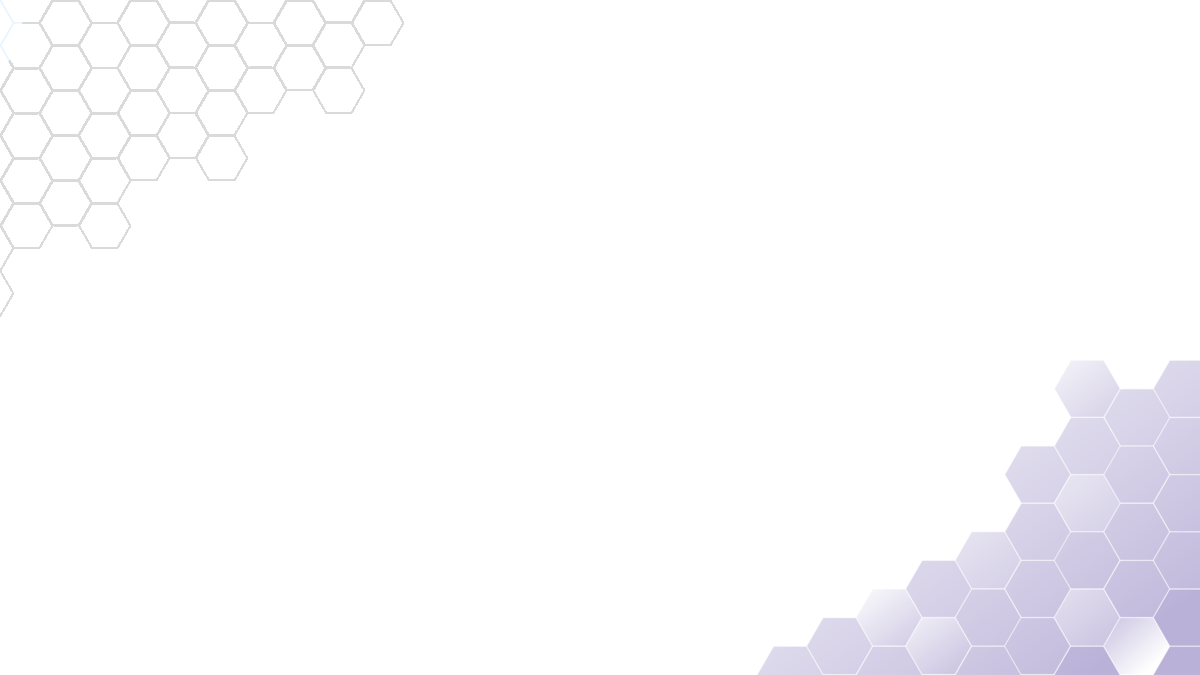
\includegraphics[width=\paperwidth,height=\paperheight]{figures/beamer-model-7-background.png}%
}

\title{Alergia Algorithm: Simulation \& Implementation}
\subtitle{Automata Modeling for DNA Sequence Representation}
\author{Your Name}
\institute{BUET}
\date{\today}

\begin{document}

% ---------------------------------------------------------------
\begin{frame}
  \titlepage
\end{frame}

% ---------------------------------------------------------------
\begin{frame}{Where We Are}
  \begin{itemize}
    \item Previous part: built a \textbf{Prefix Tree Acceptor (PTA)} directly
          from training strings
    \item The PTA is \textbf{rigid} --- it accepts only the exact strings it
          was built from
    \item DNA sequences carry point mutations, so we need something that
          \textbf{generalizes}
    \item This part: the \textbf{Alergia algorithm} that turns the rigid PTA
          into a compact, fault-tolerant automaton --- and a working
          simulation of it
  \end{itemize}
\end{frame}

% ---------------------------------------------------------------
\begin{frame}{The Core Idea}
  \begin{block}{One-line summary}
    Compare pairs of states statistically; if their behavior is
    indistinguishable within a confidence bound, \textbf{merge} them.
    Repeat until no more merges are possible.
  \end{block}
  \vspace{0.5cm}
  \begin{itemize}
    \item Each state tracks: how many strings pass through it, how many
          take each next symbol, how many end there
    \item Two states are \textbf{compatible} if these statistics agree
          within a confidence parameter $\alpha$
    \item Compatible states get merged, and their subtrees are folded
          together
  \end{itemize}
\end{frame}

% ---------------------------------------------------------------
% Fig. 7 only has ONE box for the whole Alergia algorithm ("Generate
% SFA"), so a line-by-line mapping needs a finer-grained flowchart of
% just that step. This one is derived directly from the pseudocode
% itself (Fig. 4) rather than copied from the paper.
\begin{frame}{Algorithm Alergia $\leftrightarrow$ the Flow}
\begin{columns}[T]

% ---- LEFT: mini flowchart of just the Alergia step, with a highlight
% box that jumps to a different node on each overlay step ----
\begin{column}{0.44\textwidth}
  \begin{center}
  \resizebox{!}{0.78\textheight}{%
  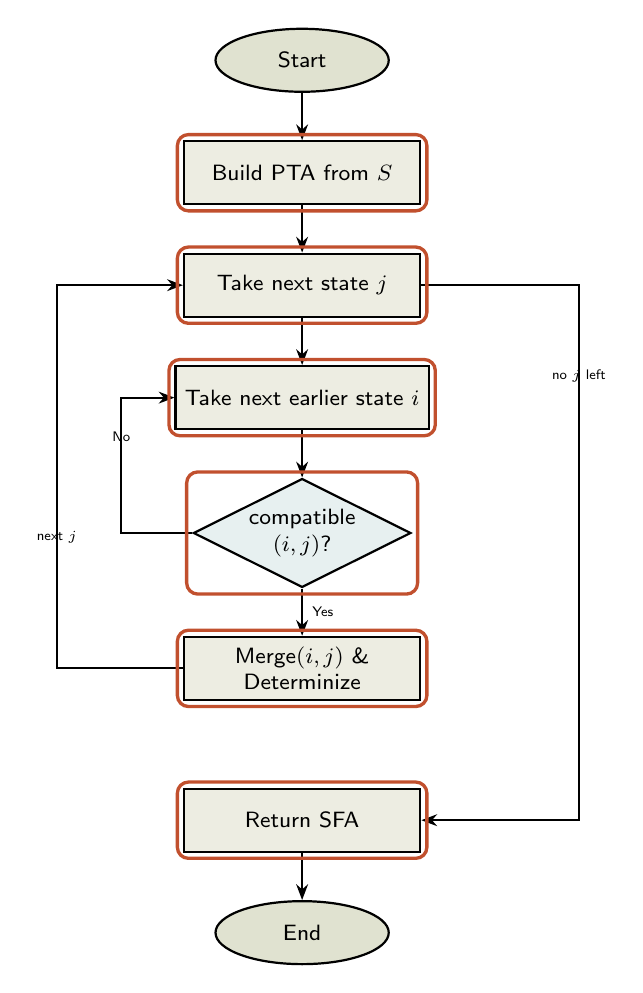
\begin{tikzpicture}[node distance=6mm and 6mm]
    \tikzstyle{startstop} = [ellipse, draw, thick, fill=oliveGreen!15!olivePaper,
      minimum width=2.2cm, minimum height=0.8cm, font=\footnotesize, align=center]
    \tikzstyle{process} = [rectangle, draw, thick, fill=oliveGreen!7!olivePaper,
      minimum width=3.0cm, minimum height=0.8cm, font=\footnotesize, align=center]
    \tikzstyle{decision} = [diamond, draw, thick, fill=oliveTealBg, aspect=2,
      minimum width=2.6cm, minimum height=1.0cm, font=\footnotesize, align=center, inner sep=1pt]
    \tikzstyle{arrow} = [thick, -{Stealth[length=2mm]}]

    \node (start)     [startstop] {Start};
    \node (buildpta)  [process, below=of start] {Build PTA from $S$};
    \node (loopj)     [process, below=of buildpta] {Take next state $j$};
    \node (loopi)     [process, below=of loopj] {Take next earlier state $i$};
    \node (compat)    [decision, below=of loopi] {compatible\\$(i,j)$?};
    \node (mergestep) [process, below=of compat] {Merge$(i,j)$ \&\\ Determinize};
    \node (returnsfa) [process, below=of mergestep, yshift=-0.5cm] {Return SFA};
    \node (end)       [startstop, below=of returnsfa] {End};

    \draw [arrow] (start) -- (buildpta);
    \draw [arrow] (buildpta) -- (loopj);
    \draw [arrow] (loopj) -- (loopi);
    \draw [arrow] (loopi) -- (compat);
    \draw [arrow] (compat.west) -- ++(-0.9,0) |- node[pos=0.3, above, font=\tiny]{No} (loopi.west);
    \draw [arrow] (compat) -- node[right, font=\tiny]{Yes} (mergestep);
    \draw [arrow] (mergestep.west) -- ++(-1.6,0) |- node[pos=0.15, above, font=\tiny]{next $j$} (loopj.west);
    \draw [arrow] (loopj.east) -- ++(2.0,0) |- node[pos=0.1, above, font=\tiny]{no $j$ left} (returnsfa.east);
    \draw [arrow] (returnsfa) -- (end);

    % ---- highlight box: jumps to a different node on each step ----
    \node<1>[draw=oliveRust, very thick, fit=(buildpta), inner sep=2pt, rounded corners] {};
    \node<2>[draw=oliveRust, very thick, fit=(loopj), inner sep=2pt, rounded corners] {};
    \node<3>[draw=oliveRust, very thick, fit=(loopi), inner sep=2pt, rounded corners] {};
    \node<4>[draw=oliveRust, very thick, fit=(compat), inner sep=2pt, rounded corners] {};
    \node<5>[draw=oliveRust, very thick, fit=(mergestep), inner sep=2pt, rounded corners] {};
    \node<6>[draw=oliveRust, very thick, fit=(returnsfa), inner sep=2pt, rounded corners] {};
  \end{tikzpicture}%
  }
  \end{center}
\end{column}

% ---- RIGHT: the pseudocode, revealed in the same 6 steps ----
\begin{column}{0.53\textwidth}
  \small
  \uncover<1->{%
    \textbf{Input:} $S$, $\alpha$ \quad \textbf{Output:} SFA\\
    $A \gets$ stochastic PTA from $S$\\[6pt]
  }
  \uncover<2->{%
    \textbf{for} $j$ = successor(firstnode($A$)) \textbf{to} lastnode($A$):\\[4pt]
  }
  \uncover<3->{%
    \hspace{0.5cm}\textbf{for} $i$ = firstnode($A$) \textbf{to} $j$:\\[4pt]
  }
  \uncover<4->{%
    \hspace{1.0cm}\textbf{if} compatible($i,j$):\\[4pt]
  }
  \uncover<5->{%
    \hspace{1.5cm}merge($A, i, j$)\\
    \hspace{1.5cm}determinize($A$)\\
    \hspace{1.5cm}exit $i$ loop\\[4pt]
  }
  \uncover<6->{%
    \textbf{return} $A$
  }
\end{column}
\end{columns}
\end{frame}

% ---------------------------------------------------------------
\begin{frame}{Compatibility Test}
  Two states are compared using a Hoeffding-bound based confidence test:
  \[
    \left| \frac{f}{n} - \frac{f'}{n'} \right|
    \;>\;
    \sqrt{\tfrac{1}{2}\log\tfrac{2}{\alpha}\left(\tfrac{1}{\sqrt{n}} + \tfrac{1}{\sqrt{n'}}\right)}
  \]
  \vspace{0.3cm}
  \begin{itemize}
    \item $n, n'$ = number of strings arriving at each state
    \item $f, f'$ = number of strings ending / following a given transition
    \item If the left side exceeds the right side, the states are
          \textbf{different} --- otherwise they are merge candidates
  \end{itemize}
  \vspace{0.3cm}
  \begin{alertblock}{Key takeaway}
    Lower $\alpha$ $\rightarrow$ looser test $\rightarrow$ more merging
    $\rightarrow$ more generalization (more mutation-tolerant).
  \end{alertblock}
\end{frame}

% ---------------------------------------------------------------
\begin{frame}{Recursive Compatibility Check}
  Compatibility is not just local --- it is checked \textbf{recursively}
  down the subtree:
  \begin{itemize}
    \item States $i$ and $j$ must agree on ending-frequency and
          every symbol's transition frequency
    \item Their destination states (children) must \emph{also} be
          compatible, all the way down
    \item Only if the whole subtree agrees are $i$ and $j$ merged
  \end{itemize}
  \vspace{0.3cm}
  \centering
  \textit{This is why merging two states can cascade into merging several
  more states at once.}
\end{frame}

% ---------------------------------------------------------------
\begin{frame}{The Full Pipeline (Paper's Fig.\ 7)}
\begin{columns}[T]

% ---- LEFT: single-column flowchart (reflowed from the paper's 2-column
% version so it fits a narrow panel), with a highlight box that jumps
% to a different node on each overlay step ----
\begin{column}{0.42\textwidth}
  \begin{center}
  \resizebox{!}{0.78\textheight}{%
  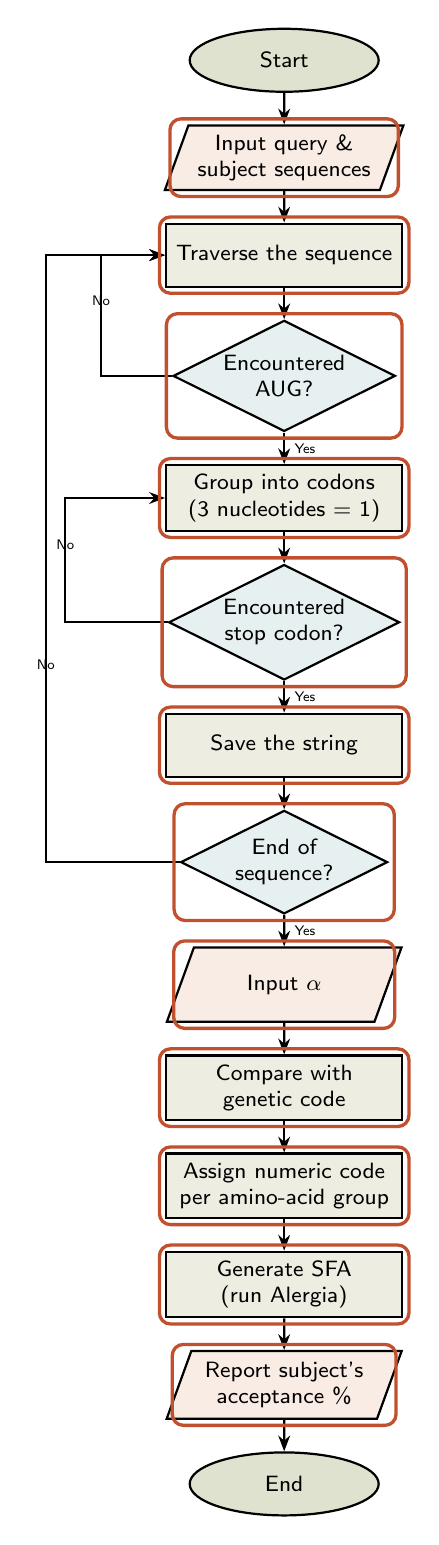
\begin{tikzpicture}[node distance=4mm]
    \tikzstyle{startstop} = [ellipse, draw, thick, fill=oliveGreen!15!olivePaper,
      minimum width=2.4cm, minimum height=0.8cm, font=\footnotesize, align=center]
    \tikzstyle{io} = [trapezium, trapezium left angle=70, trapezium right angle=110,
      draw, thick, fill=oliveRustBg, minimum width=3.0cm, minimum height=0.8cm,
      font=\footnotesize, align=center]
    \tikzstyle{process} = [rectangle, draw, thick, fill=oliveGreen!7!olivePaper,
      minimum width=3.0cm, minimum height=0.8cm, font=\footnotesize, align=center]
    \tikzstyle{decision} = [diamond, draw, thick, fill=oliveTealBg, aspect=2,
      minimum width=2.6cm, minimum height=0.95cm, font=\footnotesize, align=center, inner sep=1pt]
    \tikzstyle{arrow} = [thick, -{Stealth[length=2mm]}]

    \node (start)    [startstop] {Start};
    \node (input)    [io, below=of start] {Input query \&\\ subject sequences};
    \node (traverse) [process, below=of input] {Traverse the sequence};
    \node (aug)      [decision, below=of traverse] {Encountered\\ AUG?};
    \node (group)    [process, below=of aug] {Group into codons\\ (3 nucleotides = 1)};
    \node (stop)     [decision, below=of group] {Encountered\\ stop codon?};
    \node (save)     [process, below=of stop] {Save the string};
    \node (endseq)   [decision, below=of save] {End of\\ sequence?};
    \node (alpha)    [io, below=of endseq] {Input $\alpha$};
    \node (compare)  [process, below=of alpha] {Compare with\\ genetic code};
    \node (assign)   [process, below=of compare] {Assign numeric code\\ per amino-acid group};
    \node (sfa)      [process, below=of assign] {Generate SFA\\ (run Alergia)};
    \node (accept)   [io, below=of sfa] {Report subject's\\ acceptance \%};
    \node (end)      [startstop, below=of accept] {End};

    \draw [arrow] (start) -- (input);
    \draw [arrow] (input) -- (traverse);
    \draw [arrow] (traverse) -- (aug);
    \draw [arrow] (aug) -- node[right, font=\tiny]{Yes} (group);
    \draw [arrow] (aug.west) -- ++(-0.9,0) |- node[pos=0.25, above, font=\tiny]{No} (traverse.west);
    \draw [arrow] (group) -- (stop);
    \draw [arrow] (stop) -- node[right, font=\tiny]{Yes} (save);
    \draw [arrow] (stop.west) -- ++(-1.3,0) |- node[pos=0.25, above, font=\tiny]{No} (group.west);
    \draw [arrow] (save) -- (endseq);
    \draw [arrow] (endseq.west) -- ++(-1.7,0) |- node[pos=0.15, above, font=\tiny]{No} (traverse.west);
    \draw [arrow] (endseq) -- node[right, font=\tiny]{Yes} (alpha);
    \draw [arrow] (alpha) -- (compare);
    \draw [arrow] (compare) -- (assign);
    \draw [arrow] (assign) -- (sfa);
    \draw [arrow] (sfa) -- (accept);
    \draw [arrow] (accept) -- (end);

    % ---- highlight box: jumps to a different node on each step ----
    \node<1>[draw=oliveRust, very thick, fit=(input), inner sep=2pt, rounded corners] {};
    \node<2>[draw=oliveRust, very thick, fit=(traverse), inner sep=2pt, rounded corners] {};
    \node<3>[draw=oliveRust, very thick, fit=(aug), inner sep=2pt, rounded corners] {};
    \node<4>[draw=oliveRust, very thick, fit=(group), inner sep=2pt, rounded corners] {};
    \node<5>[draw=oliveRust, very thick, fit=(stop), inner sep=2pt, rounded corners] {};
    \node<6>[draw=oliveRust, very thick, fit=(save), inner sep=2pt, rounded corners] {};
    \node<7>[draw=oliveRust, very thick, fit=(endseq), inner sep=2pt, rounded corners] {};
    \node<8>[draw=oliveRust, very thick, fit=(alpha), inner sep=2pt, rounded corners] {};
    \node<9>[draw=oliveRust, very thick, fit=(compare), inner sep=2pt, rounded corners] {};
    \node<10>[draw=oliveRust, very thick, fit=(assign), inner sep=2pt, rounded corners] {};
    \node<11>[draw=oliveRust, very thick, fit=(sfa), inner sep=2pt, rounded corners] {};
    \node<12>[draw=oliveRust, very thick, fit=(accept), inner sep=2pt, rounded corners] {};
  \end{tikzpicture}%
  }
  \end{center}
\end{column}

% ---- RIGHT: one short description at a time, matching the highlighted box ----
\begin{column}{0.55\textwidth}
  \vspace{2cm}
  \only<1>{\normalsize Read in the query and subject DNA/RNA sequences to be compared.}
  \only<2>{\normalsize Scan through the sequence one base at a time.}
  \only<3>{\normalsize Keep scanning until the start codon AUG is found --- that's where translation begins.}
  \only<4>{\normalsize From AUG onward, group every 3 bases into one codon.}
  \only<5>{\normalsize Keep grouping codons until a stop codon (UAA, UAG, or UGA) appears.}
  \only<6>{\normalsize Save the completed codon string for this region.}
  \only<7>{\normalsize If sequence remains, go back and look for the next AUG.}
  \only<8>{\normalsize Choose the confidence parameter $\alpha$, which controls how loosely states may merge.}
  \only<9>{\normalsize Look up each codon's amino acid using the standard genetic code table.}
  \only<10>{\normalsize Replace each codon with its polarity-group number (0--3, or $-1$ for a stop codon).}
  \only<11>{\normalsize Run the Alergia algorithm on the codon strings to build the automaton.}
  \only<12>{\normalsize Test the subject sequence against the automaton and report its acceptance \%.}
\end{column}

\end{columns}
\end{frame}

% ---------------------------------------------------------------
\begin{frame}{Simulation: What We Built}
  \begin{itemize}
    \item A from-scratch Python implementation of the full pipeline:
          PTA construction $\to$ compatibility test $\to$ recursive merge/fold
    \item \textbf{Verified for correctness} against the paper's own worked
          example (its Table 1, and its 10-string toy training set)
    \item Our simulation reproduces:
      \begin{itemize}
        \item the exact same per-state frequency statistics as the paper's Table 1
        \item the exact same final acceptance rate (\textbf{40\%}) on the paper's
              own test set $Q$
      \end{itemize}
  \end{itemize}
\end{frame}

% ---------------------------------------------------------------
\begin{frame}{Simulation: Initial PTA}
  \begin{columns}[c]
    \begin{column}{0.58\textwidth}
      \centering
      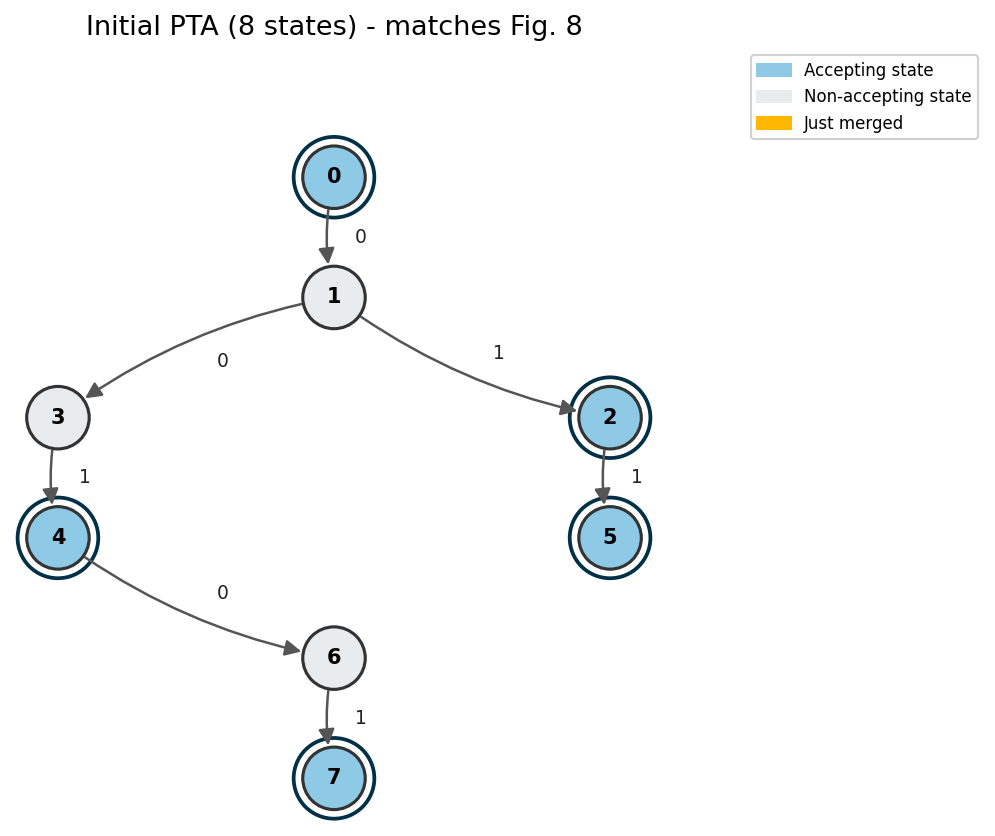
\includegraphics[height=5.2cm]{figures/toy_step0_pta.png}
    \end{column}
    \begin{column}{0.40\textwidth}
      \begin{block}{}
        \small Training set:\\[4pt]
        $S = \{\lambda,\lambda,01,01,$\\
        $001,001,001,011,$\\
        $00101,00101\}$\\[8pt]
        8 states --- matches the paper's Fig.\ 8 exactly.
      \end{block}
    \end{column}
  \end{columns}
\end{frame}

% ---------------------------------------------------------------
\begin{frame}{Simulation: Merge 1 of 4}
  \begin{columns}[c]
    \begin{column}{0.58\textwidth}
      \centering
      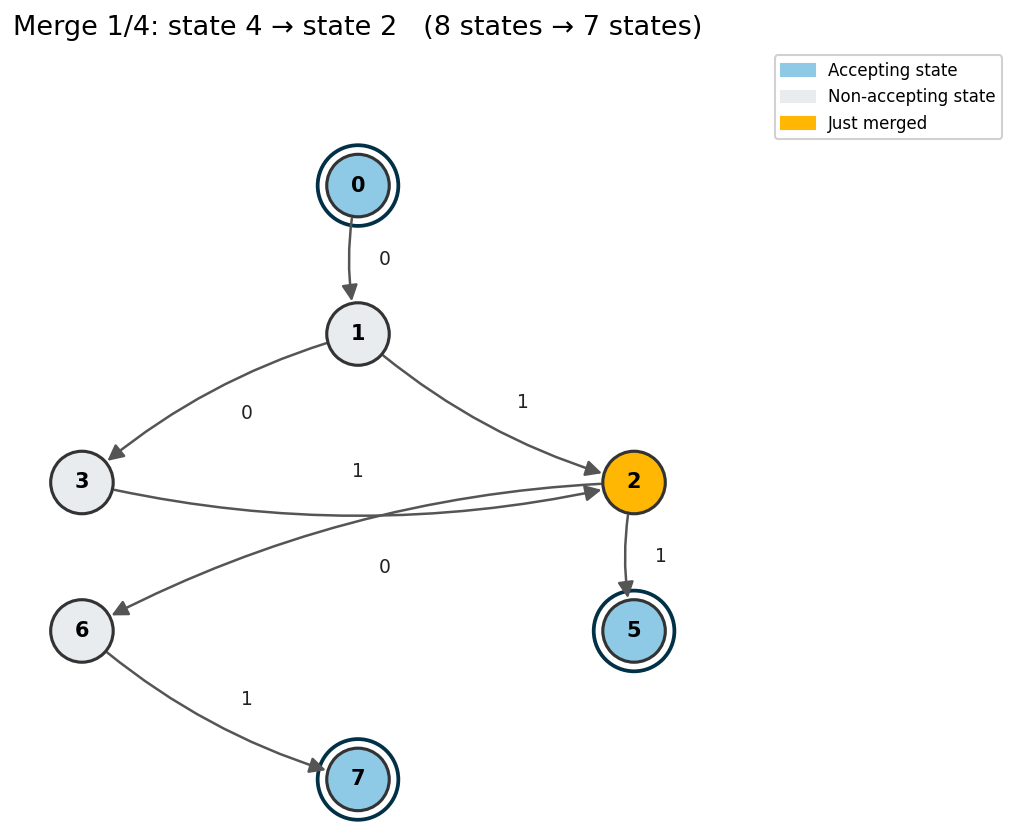
\includegraphics[height=5.2cm]{figures/toy_step1.png}
    \end{column}
    \begin{column}{0.40\textwidth}
      \begin{block}{}
        \normalsize 8 states $\to$ 7 states.
      \end{block}
    \end{column}
  \end{columns}
\end{frame}

% ---------------------------------------------------------------
\begin{frame}{Simulation: Merge 2 of 4}
  \begin{columns}[c]
    \begin{column}{0.58\textwidth}
      \centering
      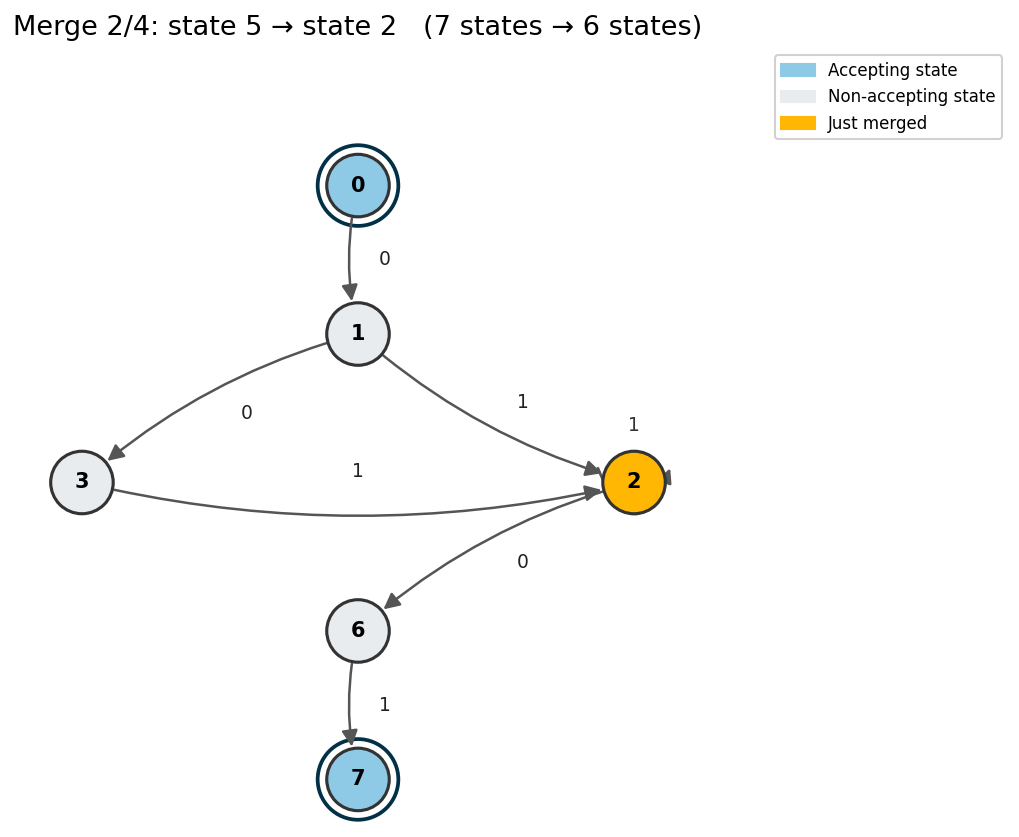
\includegraphics[height=5.2cm]{figures/toy_step2.png}
    \end{column}
    \begin{column}{0.40\textwidth}
      \begin{block}{}
        \normalsize 7 states $\to$ 6 states.
      \end{block}
    \end{column}
  \end{columns}
\end{frame}

% ---------------------------------------------------------------
\begin{frame}{Simulation: Merge 3 of 4 --- a Cascade}
  \begin{columns}[c]
    \begin{column}{0.58\textwidth}
      \centering
      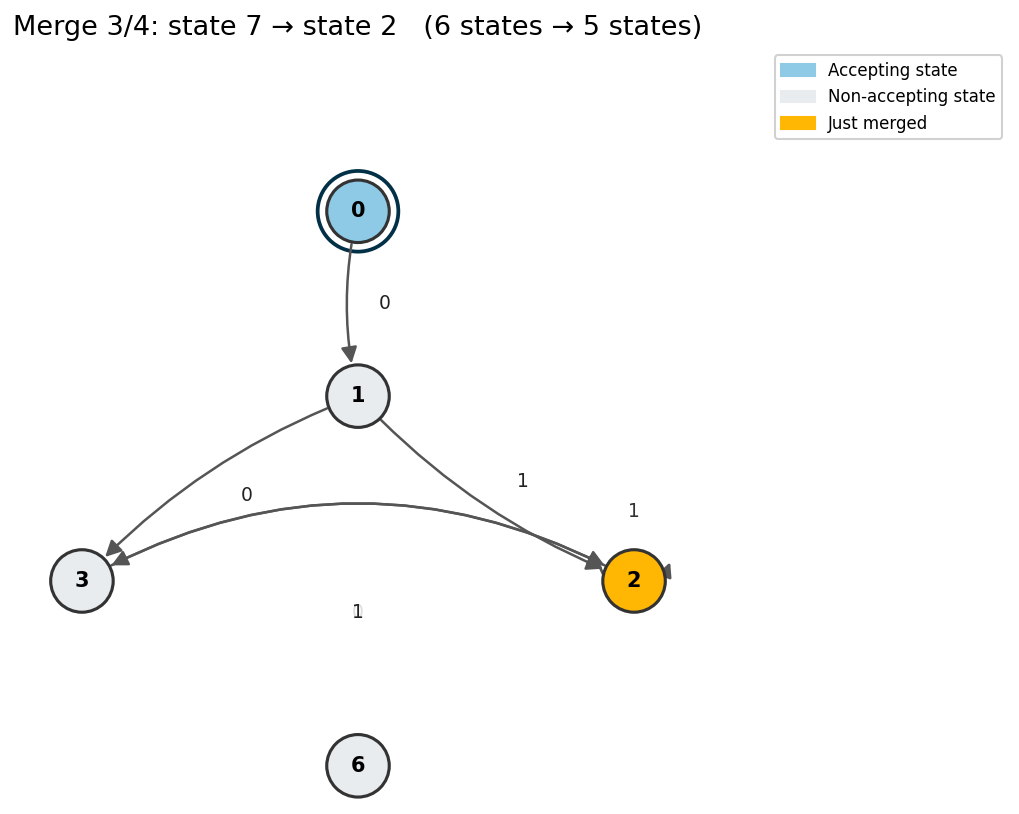
\includegraphics[height=5.2cm]{figures/toy_step3.png}
    \end{column}
    \begin{column}{0.40\textwidth}
      \begin{block}{}
        \small 6 states $\to$ 5 states.\\[8pt]
        This merge was triggered internally while resolving Merge 4 ---
        one compatibility decision pulled two states together at once.
      \end{block}
    \end{column}
  \end{columns}
\end{frame}

% ---------------------------------------------------------------
\begin{frame}{Simulation: Final Automaton}
  \begin{columns}[c]
    \begin{column}{0.58\textwidth}
      \centering
      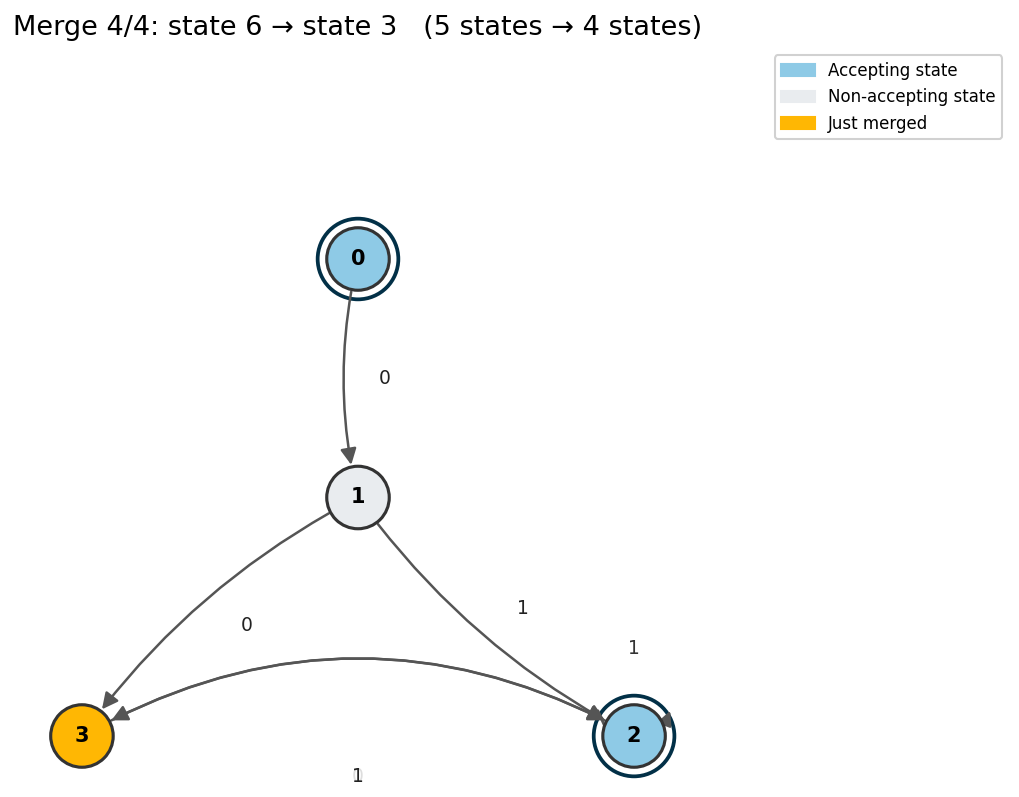
\includegraphics[height=5.2cm]{figures/toy_step4.png}
    \end{column}
    \begin{column}{0.40\textwidth}
      \begin{block}{}
        \small 8 states $\to$ 4 states, in 4 real merge steps.\\[8pt]
        Acceptance rate on test set $Q$: \textbf{40\%} (matches the paper exactly).
      \end{block}
    \end{column}
  \end{columns}
\end{frame}

% ---------------------------------------------------------------
\begin{frame}{Simulation: Applying It to DNA-Style Data}
  \begin{itemize}
    \item Same pipeline, now run on codon-group strings from the paper's own
          DNA example (Chapter 4 training strings)
    \item Initial PTA: \textbf{80 states}
  \end{itemize}
  \vspace{0.3cm}
  \begin{center}
  \begin{tabular}{ccc}
    \toprule
    $\alpha$ & Merge events & Final states \\
    \midrule
    0.7 (strict) & 8  & 72 \\
    0.5          & 70 & 10 \\
    0.3 (loose)  & 78 & 2  \\
    \bottomrule
  \end{tabular}

  \vspace{0.3cm}
  \small Lower $\alpha$ $\rightarrow$ dramatically more generalization.
  \end{center}
\end{frame}

% ---------------------------------------------------------------
\begin{frame}{Simulation: DNA Automaton at $\alpha = 0.3$}
  \begin{columns}[c]
    \begin{column}{0.58\textwidth}
      \centering
      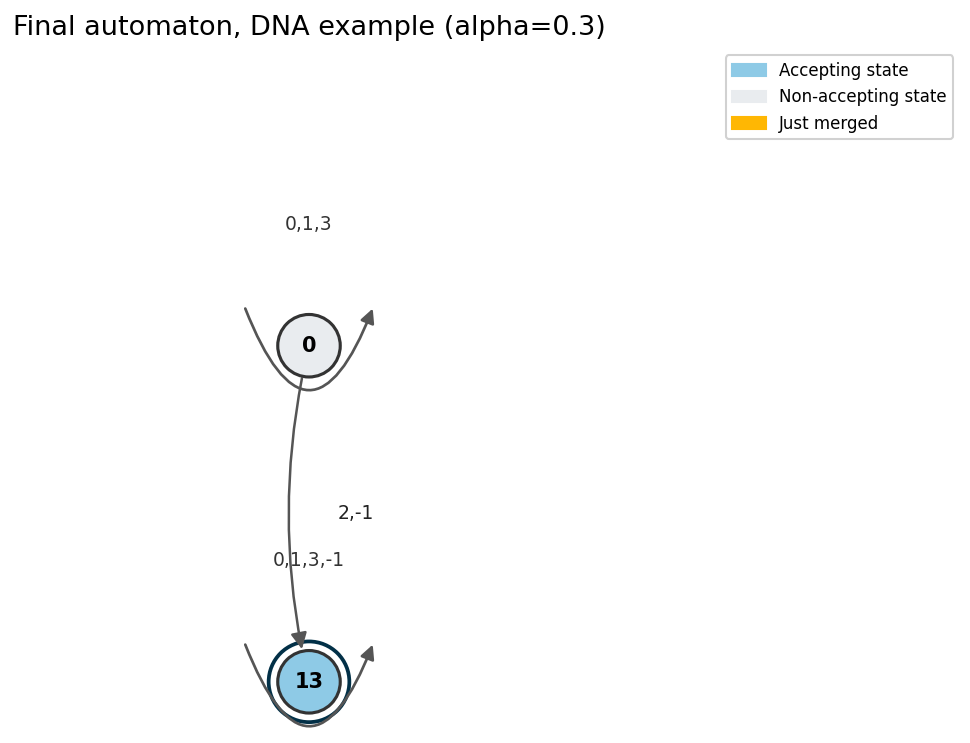
\includegraphics[height=5.2cm]{figures/dna_final_alpha03.png}
    \end{column}
    \begin{column}{0.40\textwidth}
      \begin{block}{}
        \small At very loose $\alpha$, 80 states collapse into just 2 ---
        almost everything becomes self-loops on one accepting state.
      \end{block}
    \end{column}
  \end{columns}
\end{frame}

% ---------------------------------------------------------------
\begin{frame}{Live Demo: Watch It Merge}
  \begin{itemize}
    \item These slides show discrete steps --- the live demo also has two
          \textbf{animated} versions, played outside the slides:
    \item \texttt{toy\_merge\_animation.gif} --- the 4-step example above,
          playing start to finish
    \item \texttt{dna\_merge\_animation.gif} --- the DNA automaton actually
          shrinking, merge by merge, from 80 states down to 10
  \end{itemize}
\end{frame}

% ---------------------------------------------------------------
\begin{frame}{Implementation Overview (Java)}
  Built in Java (Eclipse): \texttt{AminoView.java} (I/O) +
  \texttt{Train.java} (algorithm logic).
  \vspace{0.2cm}
  \small
  \begin{tabular}{ll}
    \toprule
    \textbf{Function} & \textbf{Role} \\
    \midrule
    \texttt{GetCodons()} & Parses DNA into codon-group symbols \\
    \texttt{CreatePTA()} & Builds the initial prefix tree \\
    \texttt{Compatible() / Differ()} & The statistical merge-decision test \\
    \texttt{Delta(i, t)} & Transition lookup (state $\times$ symbol $\to$ state) \\
    \texttt{Combine() / MergeAll()} & Performs the merges, updates statistics \\
    \bottomrule
  \end{tabular}
\end{frame}

% ---------------------------------------------------------------
\begin{frame}{Summary}
  \begin{itemize}
    \item Alergia turns a rigid PTA into a compact, mutation-tolerant
          automaton by statistically merging equivalent states
    \item The confidence parameter $\alpha$ directly controls how much the
          automaton generalizes
    \item Our simulation reproduces the paper's own results exactly,
          confirming the implementation is correct
    \item Same pipeline applies directly to DNA codon-group sequences
  \end{itemize}
\end{frame}

\end{document}
